\chapter{Topology: twin states, boundaries and loops}
\label{ch:topology}

\section{The three twin states}

A triangle mesh distributed over ranks has three kinds of ``edges without a stored
neighbour'' that must never be confused: the physical boundary of an open surface, the edge of
this rank's part of the mesh (the MPI rim), and --- on a periodic domain --- the crossing of a
periodic face. \mftl{} separates them by giving every half-edge exactly one of three
\emph{twin states} at every quiescent point:

\begin{center}\small
\begin{tabular}{@{}llll@{}}
\toprule
State & \texttt{twin\_idx} & \texttt{twin\_gid} & Meaning \\
\midrule
LOCAL & $\ge 0$ & global id of the stored twin & the twin is stored on this rank \\
REMOTE & $-1$ & $\ge 0$: global id of the twin & the twin lives on another rank (MPI rim) \\
BOUNDARY & $-1$ & $-2-\text{tag}$, $\text{tag}\ge0$ & a physical boundary edge with a tag \\
\bottomrule
\end{tabular}
\end{center}

\texttt{MFTL\_TWIN\_NONE} is $-2$, so the boundary code of tag $t$ is
$\fn{MFTLBoundaryCode}(t)=-2-t$. The transient value \texttt{MFTL\_TWIN\_UNKNOWN} ($-1$) is legal
only inside an operation (a remesh pass, a staged copy) and is rejected by validation. The
states are read with the predicates of \texttt{mftl\_topology.h} only:

\begin{lstlisting}[numbers=none]
bool MFTLHeIsLocal(const MFTL_HalfEdge *he);
bool MFTLHeIsRemote(const MFTL_HalfEdge *he);
bool MFTLHeIsBoundary(const MFTL_HalfEdge *he);
int  MFTLHeBoundaryTag(const MFTL_HalfEdge *he);                 /* BOUNDARY only */
int  MFTLHeTwinGid(const MFTL_Object *obj, const MFTL_HalfEdge *he); /* -1 for BOUNDARY */
int  MFTLHeEdgeId(const MFTL_Object *obj, const MFTL_HalfEdge *he);  /* undirected edge id */
\end{lstlisting}
\fn{MFTLHeEdgeId} is the rank-independent id of the undirected edge: the smaller of the two
half-edge ids for LOCAL and REMOTE edges, the half-edge's own id for a boundary edge.

\section{Boundary, rim and seam}
\label{sec:bound-rim-seam}

Table~\ref{tab:brs} states the distinction precisely. No coordinate is ever consulted to decide
it: the physical boundary is a property of the topology, the rim a property of the
distribution, and the seam a property of the image counters.

\begin{table}[ht]
\centering\small
\begin{tabularx}{\textwidth}{@{}lXX@{}}
\toprule
Concept & Representation & Determined by \\
\midrule
Physical boundary & BOUNDARY half-edge (\texttt{twin\_idx} $=-1$, \texttt{twin\_gid} $\le -2$) & the topology only: builders, commits, remesh operators \\
MPI rim & REMOTE half-edge (\texttt{twin\_idx} $=-1$, \texttt{twin\_gid} $\ge0$), with a live twin on another rank & the ownership and ghosting only \\
Periodic seam & ordinary LOCAL or REMOTE twins; the crossing shows only in the edge lattice shift derived from the image counters (\S\ref{sec:winding}) & the topology plus the counters \\
\bottomrule
\end{tabularx}
\caption{Physical boundary, MPI rim and periodic seam.}
\label{tab:brs}
\end{table}

The concepts compose: an edge across a periodic seam may also be an MPI rim; a physical
boundary may run across seams and rank boundaries --- its half-edges are BOUNDARY on every rank,
and its loop is built collectively (\S\ref{sec:loops}).

\begin{figure}[ht]
\centering
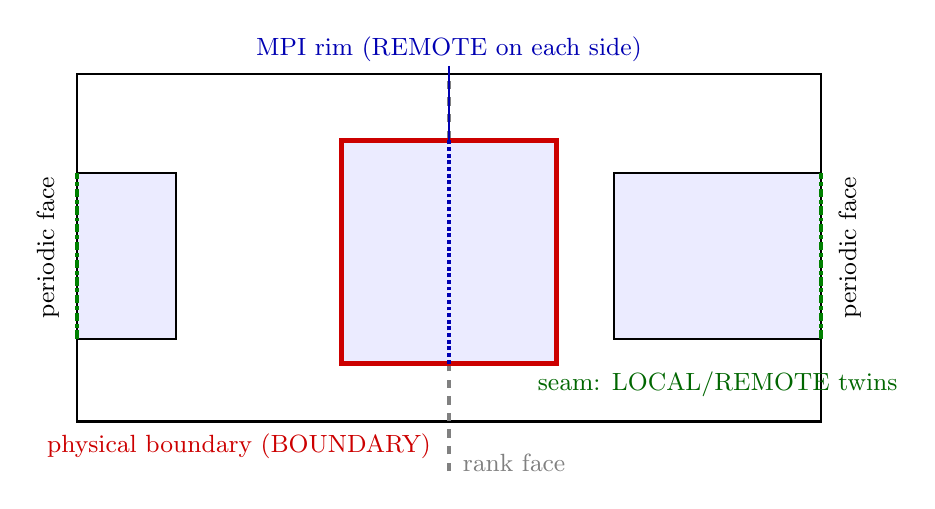
\begin{tikzpicture}[scale=1.05]
  \draw[thick] (0,0) rectangle (9,4.2);
  \draw[very thick,dashed,gray] (4.5,-0.6) -- (4.5,4.2); \node[gray,font=\small,right] at (4.55,-0.5) {rank face};
  \node[font=\small] at (-0.35,2.1) [rotate=90] {periodic face};
  \node[font=\small] at (9.35,2.1) [rotate=90] {periodic face};
  % an open patch crossing the rank face and the periodic face
  \draw[fill=blue!8,thick] (6.5,1) -- (9,1) -- (9,3) -- (6.5,3) -- cycle;
  \draw[fill=blue!8,thick] (0,1) -- (1.2,1) -- (1.2,3) -- (0,3) -- cycle;
  \draw[fill=blue!8] (3.2,0.7) -- (5.8,0.7) -- (5.8,3.4) -- (3.2,3.4) -- cycle;
  \draw[red!80!black,line width=1.6pt] (3.2,0.7) -- (5.8,0.7) -- (5.8,3.4) -- (3.2,3.4) -- cycle;
  \draw[blue!70!black,line width=1.4pt,densely dotted] (4.5,0.7) -- (4.5,3.4);
  \draw[green!50!black,line width=1.4pt,densely dashdotted] (9,1) -- (9,3); \draw[green!50!black,line width=1.4pt,densely dashdotted] (0,1) -- (0,3);
  \node[font=\small,red!80!black,left] at (4.4,-0.3) {physical boundary (BOUNDARY)};
  \node[font=\small,blue!70!black] at (4.5,4.5) {MPI rim (REMOTE on each side)};
  \draw[blue!70!black,thin] (4.5,4.3) -- (4.5,3.4);
  \node[font=\small,green!40!black,align=center] at (7.75,0.45) {seam: LOCAL/REMOTE twins};
\end{tikzpicture}
\caption{The three situations in which a rank stores no twin across an edge, or in which an
edge crosses the box: a physical boundary (a tagged BOUNDARY half-edge), an MPI rim (REMOTE
half-edges whose twins live on the neighbouring rank) and a periodic seam (ordinary twins; the
crossing is visible only through the image counters).}
\label{fig:brs}
\end{figure}

\section{Declared class: closed and open bodies}

A body is closed unless the application declares it open, identically on every rank, before
it is built:
\begin{lstlisting}[numbers=none]
void MFTLObjectDeclareOpen(MFTL_Object *obj, int open);
\end{lstlisting}
Only a declared-open body may have BOUNDARY half-edges. An unmatched edge in the input of a
closed body is an error, never a silently created boundary. The declared class, the boundary
tags and the image counters are the only information from which the library derives what a
body is; geometric proximity to the box faces plays no role.

\section{Building a mesh}

\paragraph{From vertex positions and index triples (rank-local).}\mbox{}
\begin{lstlisting}[numbers=none]
int MFTLBuildTopologyFromTriples(MFTL_Object *obj, int nV, const double positions[][3],
                                 int nF, const int triples[][3]);
\end{lstlisting}
For a triple $(a,b,c)$ the three half-edges target $b$, $c$ and $a$ and cycle in that order, so
the winding of the triples defines the orientation. Twins are paired locally; on a declared-open
body every unpaired half-edge becomes BOUNDARY, with tags numbering the boundary loops in the
order of their smallest vertex id; on a closed body an unpaired half-edge is an error. Duplicate
directed half-edges (a non-manifold edge, inconsistent orientation, a M\"obius strip) and bow-tie
vertices are rejected. Positions are stored as given with \texttt{img} $=0$; a caller with
continuous coordinates wraps them first. The generators and the readers use this path.

\paragraph{From a distributed triangle soup (collective).}\mbox{}
\begin{lstlisting}[numbers=none]
int MFTLBuildFromSoup(MFTL_Object *obj, int nV, const int *vgid, const double (*pos)[3],
                      const int *vowner, int nT, const int *tgid, const int (*tvg)[3],
                      const int *towner);
int MFTLBuildFromSoupEx(/* as above */ ..., const MFTL_BoundaryDecl *decl);
int MFTLBuildFromSoupImg(/* wrapped positions with image counters */ ...);
\end{lstlisting}
Every rank passes the vertices and triangles it knows, with global ids; a triangle names its
vertices by global id, and the order of its three vertex ids defines its orientation. An
entity may be passed on several ranks (with identical data). Twins are paired locally, then
every unpaired half-edge is resolved \emph{globally} across ranks: if the twin exists anywhere,
the half-edge becomes REMOTE. An edge that is unmatched everywhere becomes BOUNDARY only if the
body is declared open \emph{and} the boundary declaration names it:

\begin{lstlisting}[numbers=none]
typedef struct MFTL_BoundaryEdgeDecl { int vgid_a, vgid_b; int tag; } MFTL_BoundaryEdgeDecl;
typedef struct MFTL_BoundaryDecl {
  int from_mesh;   /* "BoundaryFromMesh": every edge unmatched on every rank is a boundary */
  int n_edges;     /* or an explicit list of boundary edges with tags (union over ranks)  */
  const MFTL_BoundaryEdgeDecl *edges;
} MFTL_BoundaryDecl;
\end{lstlisting}
With \texttt{from\_mesh} the loops are tagged automatically in the order of their smallest vertex
id. Any other unmatched edge, a declared edge that is not unmatched, or a duplicate directed
half-edge is a collective error. All entities are stored with the given owners (\texttt{NULL}:
this rank); a redistribution establishes the real ownership. The example of
\S\ref{sec:ex-open} builds an open patch this way.

\paragraph{Staged copies.} \fn{MFTLObjectAppendTriangleCopy} copies a triangle (with its
half-edges, missing vertices, payload and surface scalar) from one object into another. The copy
is \emph{staged}: half-edges whose twin was not copied keep the source's state code, and the
destination is not quiescent until the batch is closed by the collective
\fn{MFTLObjectCommitCopy}\texttt{(dst, mode)}. With \texttt{MFTL\_COMMIT\_ASSEMBLE} every such
half-edge must find its twin among the destination's authoritative half-edges on some rank;
with \texttt{MFTL\_COMMIT\_CUT} the half-edges whose source twin was not copied become BOUNDARY
with one new tag (the destination must be declared open). \multi{} uses this to split a body
into its connected components (breakup) and to merge bodies (coalescence).

\section{Validation}
\label{sec:validation}

\begin{lstlisting}[numbers=none]
int MFTLCheckMeshIntegrity(MFTL_Object *object);                 /* rank-local */
int MFTLCheckTwinStatesLocal(const MFTL_Object *obj, int flags, int verbose);
int MFTLValidateTwinStatesEx(MFTL_Object *obj, int flags);       /* collective */
int MFTLValidateTwinStates(MFTL_Object *obj);
\end{lstlisting}
\fn{MFTLCheckMeshIntegrity} checks index bounds, triangle cycles, twin symmetry and vertex
consistency. \fn{MFTLCheckTwinStatesLocal} checks, rank-locally, that every live half-edge has a
legal state, that LOCAL pairs are symmetric, that only declared-open bodies have BOUNDARY
half-edges, that no directed half-edge is duplicated, and the boundary-vertex conventions; with
\texttt{MFTL\_VALIDATE\_GHOSTS} it also checks G1 and G2. \fn{MFTLValidateTwinStates} adds the
collective \emph{remote liveness} check: every REMOTE twin id is held as a live authoritative
half-edge on some rank that names the requester back, and every boundary edge carries the same
tag on every rank that stores it.

The library runs a check at every quiescent point (after builds and commits, redistribution,
remesh finalisation, the end of a serial bracket, and reading a native mesh): the full
collective validation in Debug builds or when \texttt{MFTL\_VALIDATE} is set, the cheap local
checks otherwise.

\section{Remote-twin discovery and ghost completion}
\label{sec:completion}

When a rank holds a REMOTE half-edge it knows the global id of the twin but not where it lives.
Two discovery modes find it:
\begin{itemize}
  \item \emph{Global mode} (before ownership exists: builders, commits, and as a fallback): the
    requested ids are gathered on every rank, and any rank holding a live authoritative copy
    answers.
  \item \emph{Owned mode} (after a redistribution): the twin triangle's centroid lies within
    $\ell_{\max}/3$ of the edge midpoint ($\ell_{\max}$: the longest edge), so the request goes to
    the ranks whose box meets the (periodic) ball of radius $\ell_{\max}/3+2\varepsilon$ around
    the midpoint, $\varepsilon$ being a margin for stale ghost positions. The global mode then
    always runs as a fallback (it carries no data when the first round was complete).
\end{itemize}
\fn{MFTLCompleteGhosts}, called by every redistribution, uses the discovery to import the missing
neighbours as ghosts until the two guarantees hold:
\begin{description}
  \item[G1] every edge of every owned triangle is LOCAL or BOUNDARY;
  \item[G2] the complete fan of every owned vertex is stored.
\end{description}
Kernels that work on the one-ring of an owned vertex (normals, curvature, smoothing) rely on G2;
kernels that look across the edges of an owned triangle rely on G1. Ghost triangles themselves
may keep REMOTE edges.

\section{Boundary vertices, tags and loops}
\label{sec:loops}

A \emph{boundary vertex} has exactly one outgoing and one incoming BOUNDARY half-edge; its
\texttt{out\_he\_idx} points at the outgoing one, so the loop is walked from vertex to vertex.
Tags are persistent handles for the parts of the boundary: splits inherit the tag of the split
edge, collapses along a boundary keep it, and a CUT commit creates a new one. \multi{} attaches
its boundary conditions to them (\S\ref{sec:mf-bcs}).

\begin{lstlisting}[numbers=none]
typedef struct MFTL_BoundaryLoop {
  int n;              /* number of boundary edges (= vertices) */
  int *edge_ids;      /* in loop order; edge i runs vertex_gids[i] -> vertex_gids[i+1] */
  int *vertex_gids;
  int tag;            /* the smallest tag when mixed */
  int mixed_tags;
  double length;      /* sum of minimum-image edge lengths */
  int winding[3];     /* sum of the edge lattice shifts around the loop */
} MFTL_BoundaryLoop;
int  MFTLBoundaryLoops(MFTL_Object *obj, MFTL_BoundaryLoopSet *out);   /* collective */
void MFTLFreeBoundaryLoops(MFTL_BoundaryLoopSet *set);
\end{lstlisting}
\fn{MFTLBoundaryLoops} collects one record per owned boundary vertex (its incoming and outgoing
edge ids, its id, the tag and the outgoing edge's length and lattice shift), gathers the
records on every rank and chains them into loops, ordered by their smallest vertex id. The
result is identical on every rank and independent of the rank count and of seams. It needs G2
(call it after a redistribution, or on one rank). A non-zero winding vector means the loop
itself spans a periodic direction (\S\ref{sec:winding}).

The orientation of a loop follows the half-edges: on an outward-facing patch, walking along
the boundary half-edges keeps the surface on the left. \fn{MFTLBoundaryEdgeGeometry} returns, for
a boundary half-edge, its length $L_e$, the unit tangent $\vect{t}$ along it, the in-surface
outward \emph{conormal} $\vect{\nu}=\vect{t}\times\vect{n}$ ($\vect{n}$: the unit normal of its
triangle) and the continuous midpoint (Figure~\ref{fig:conormal}).

\begin{figure}[ht]
\centering
\begin{tikzpicture}[scale=2]
  \coordinate (A) at (0,0); \coordinate (B) at (2,0); \coordinate (C) at (0.8,1.2);
  \draw[fill=gray!8] (A)--(B)--(C)--cycle;
  \draw[red!80!black,line width=1.5pt,-{Stealth[length=3mm]}] ($(C)!0.1!(A)$) -- ($(C)!0.9!(A)$);
  \node[red!80!black] at (0.18,0.75) {$h$};
  \coordinate (M) at ($(C)!0.5!(A)$);
  \draw[-{Stealth[length=2.5mm]},thick,blue!70!black] (M) -- ++(-0.45,-0.67) node[below left] {$\vect{t}$};
  \draw[-{Stealth[length=2.5mm]},thick,green!45!black] (M) -- ++(-0.62,0.42) node[left] {$\vect{\nu}$};
  \node at (1,0.4) {$T$}; \node[font=\small] at (1,0.2) {$\vect{n}$ out of page};
  \node[font=\small,align=left] at (2.9,0.9) {BOUNDARY half-edge $h$ of $T$\\ $\vect{t}$: unit tangent along $h$\\ $\vect{\nu}=\vect{t}\times\vect{n}$: outward conormal};
\end{tikzpicture}
\caption{Geometry of a boundary edge (\fn{MFTLBoundaryEdgeGeometry}).}
\label{fig:conormal}
\end{figure}
